\documentclass[Main]{subfiles}
\begin{document}

\section{General beskrivelse}
Dette afsnit giver et overblik over kravene, der er stillet for udviklingen af systemet.


\subsection{Systembeskrivelse}
Projektet vil bestå i at få en quadrocopter, af typen AeroQuad Cyclone, til autonomt at flyve imellem 3 waypoints, udstyret med en sender og en FM-trasmitter hver.
Quadrocopteren udstyres med en sender, der kan kobles på de 3 objekter, samt 3 FM-modtagere, der kan triangulere hvor ét af de 3 waypoints står. 
Quadrocopteren skal således flyve til det aktive waypoint og ved ankomst flyve til det næste objekt.
\\
For at quadrocopteren ikke støder ind i objekter på sin vej, udstyres den med 3 sonar sendere, der kan detektere forhindringer foran den, samt en sonar under den, således den ikke rammer jorden.




\subsection{Systemoversigt}

\begin{figure}[hbtp]
\centering
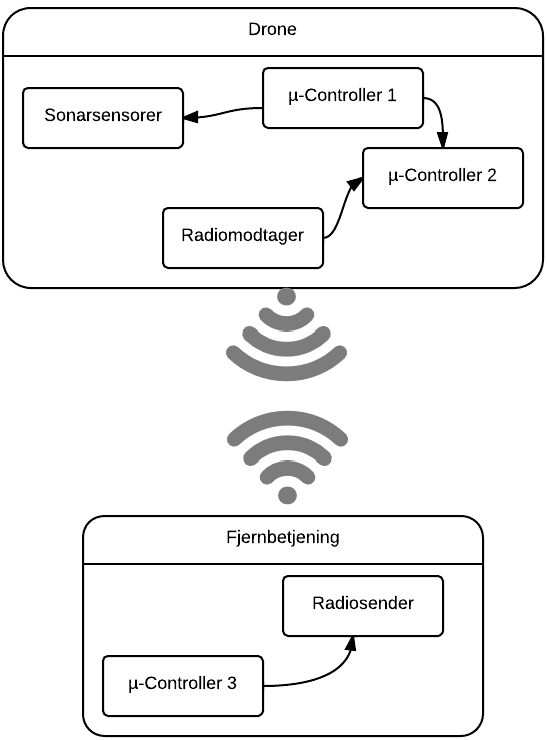
\includegraphics[scale=0.5]{Oversigt}
\caption{Systemoversigt}
\label{Fig:Oversigt}
\end{figure}

På Figur \ref{Fig:Oversigt} ses kommunikationen mellem dronen med et waypoint.
Dronen bestemmer hvilket way point den vil snakke med og sender et aktiverings-signal til alle way points.
Hvis et way point bliver forespurgt begynder dette at sende signal retur.



\subsubsection{Aktør-kontekst diagram}

På Figur \ref{Fig:Aktor-oversigt} vises aktørerne der kommunikerer med systemet.
Figuren indeholder to grupper, henholdsvis personer og hardware aktører.
Personerne der interagerer med systemet er vist på venstre side, mens de forskellige hardwaren-enheder vises på højre side.


\begin{figure}[hbtp]
\centering

\includegraphics[scale=1]{Dummy}
\caption{Systemoversigt \fxnote{Her skal indsættes en rigtigt figur}}
\label{Fig:Aktor-oversigt}
\end{figure}


\paragraph{Aktørbeskrivelser}\fxnote{Dette afspejler ikke templaten}\mbox{} \\%Dette skal bruges til line break
I det følgende beskriver en primær aktør, en aktør der har et eller flere mål, der ønskes opfyldt af systemets Use Cases. 
En sekundær aktør beskriver derimod en aktør, der er en nødvendig deltager i en eller flere Use Case for at opfylde en primær aktørs mål. 
I nogle tilfælde kan en  aktør både være primær og sekundær.

\begin{longtable}{p{0.3\textwidth}|p{0.65\textwidth}}
\hline
\textbf{Aktør navn}  				& Bruger \\
\textbf{Type} 						& Primær \\
\textbf{Beskrivelse} 				& En "Bruger" er en person, der starter og stopper dronen. \\
\textbf{Antal samtidige aktører} 	& 1 \\
\hline
\end{longtable}

\begin{longtable}{p{0.3\textwidth}|p{0.65\textwidth}}
\hline
\textbf{Aktør navn}  				& Drone \\
\textbf{Type} 						& Sekundær \\
\textbf{Beskrivelse} 				& Dronen består af AeroQuad Cyclone ARF Kit, fire sonarsensorer samt 3 FM-transceivere. \\
\textbf{Antal samtidige aktører} 	& 1 \\
\hline
\end{longtable}


\subsection{Systemets funktioner}
Systemets funktioner, de funktionelle krav, er fundet og beskrevet vha. Use Case teknikken. 
De følgende diagrammer viser systemets funktioner udtrykt som Use Cases. 
Formålet med disse diagrammer er at give et overblik over funktionaliteten i det system, der skal udvikles. 
Hver af de på diagrammerne viste Use Cases er detaljeret specificeret i kapitel \dots %\fxnote{Kapitel 3}.



\subsubsection{Use Case diagrammer}
Figur \ref{Fig:UC-Diagram} viser systemet som Use Case diagram.

\begin{figure}[hbtp]
\centering
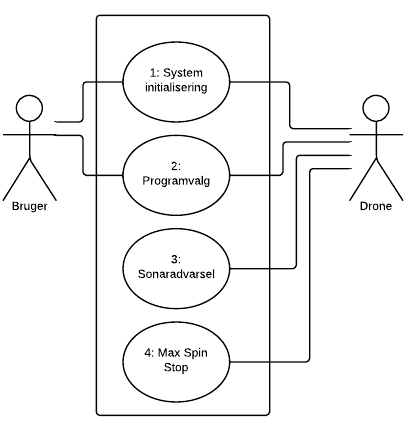
\includegraphics[scale=0.75]{UseCaseDiagram}
\caption{Use Case diagram}
\label{Fig:UC-Diagram}
\end{figure}

\end{document}